
\setcounter{section}{0}
\setcounter{figure}{0}
\graphicspath{{./figs/}{./figs/item-kneron/}}

\NewsTitle{Automatic Re-configurable Deep Neural Network Applied to Resource-Constrained Cyber-Physical Systems}
\NewsAuthor{
Chunchen Liu, Kangli Hao, Liu Liu\\
Kneron Inc.
}

\begin{abstract}
Unlike traditional embedded systems, modern cyber-physical systems (CPS) are enpowered with much stronger intelligence mechanisms proper of deep learning leading the pathway.
However, high-accuracy deep learning is very computationally intensive, which usually requires more resources than locally available.
The approach that utilizes network connectivity and cloud servers are neither suitable for hard real-time missions that bear very low latency,
nor missions that carried out in regions where network coverage is unavailable or unreliable.
This work presents the automatic reconfigurable deep neural network (ARDNN) solution,
which dramatically reduces computational requirements yet with neglectable cost of accuracy.
ARDNN enables deep convolutional multi-layer neural networks to be run on resource-constrained CPSes,
thus opens the floodgate of novel industrial, automotive, security and consumer CPS applications.
Our experimental results demonstrate that ARDNN can reduce computational cost to 1/30 with < 5\% accuracy degradation.
\end{abstract}

\section{Problem and Motivation}

Ongoing advances in science and engineering will improve the link between computational and physical elements by means of intelligent mechanisms,
dramatically increasing the functionality, adaptability, and usability of CPSes \cite{ref1}.
Recent studies have shown deep learning a.k.a. deep neural network (DNN) greatly out-performs previous techniques in accuracy when applied to the field of computer vision for object recognition (See figure below).

\begin{figure}[htbp]
	\centering
    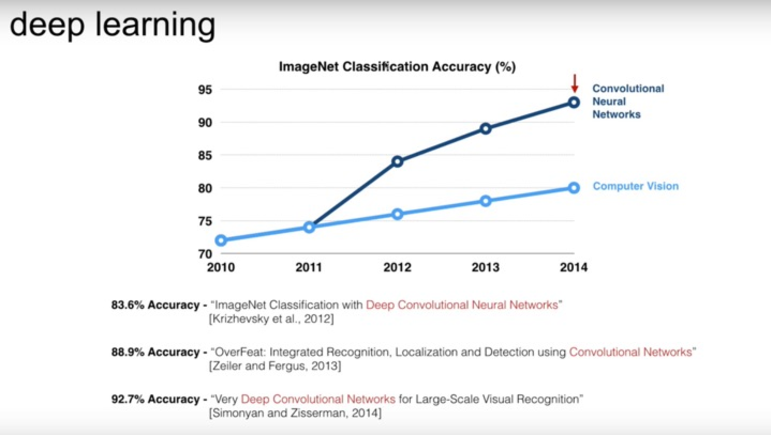
\includegraphics[width=0.64\linewidth]{fig1}
	\caption{Deep learning greatly out-performs previous techniques in image recognition accuracy.}
	\label{fig:fig1}
\end{figure}

However, deep learning models are very complex, using a cascade of many layers of nonlinear processing units for feature extraction and transformation,
which results in very heavy computational tasks that require more processor and memory resources than locally available.
For tasks that require more resources than are locally available,
one common approach for rapid implementation of mobile CPSes utilizes the network connectivity to link the CPS with either a server or a cloud environment,
enabling complex processing tasks that are impossible under local resource constraints.
However, the approach is not suitable for critical real-time missions that bear very low latency such as autonomous automotive system and unmanned aerial vehicle.
Neither suitable for missions that carried out in regions where network coverage is unavailable or unreliable, such as deep-sea exploration, search and rescue. 

Our aspiration is to design and implement an improved DNN engine on resource-constrained CPSes that can robustly and efficiently execute highly intelligent tasks.
Such a DNN engine should: 1) Execute very deep neural network on embedded device; 2) No specialized SOC or additional GPU hardware is required;
3) Training time and execution time are significantly reduced.


\section{Proposed Solution}

To drastically reduce the computational cost and time, we propose automatic reconfigurable deep neural network (ARDNN) architecture.
ARDNN is dynamic distributive architecture that can automatically and continually reconfigure the DNN cascade structure.
It can continually improve the accuracy and increase the efficiently.
We designed an improved generalization algorithm to enhance the producing of reasonable training patterns with similar but not identical input.
We resort to specialized factor variation reduction to make supervised transfer and reinforcement learning tasks much more efficient than static DNN architecture.
In addition, we use stacked RBM as deep auto-encoder and limit one layer to few dimensions to reduce the dimensionality of the ARDNN architecture. 

\begin{figure}[htbp]
	\centering
    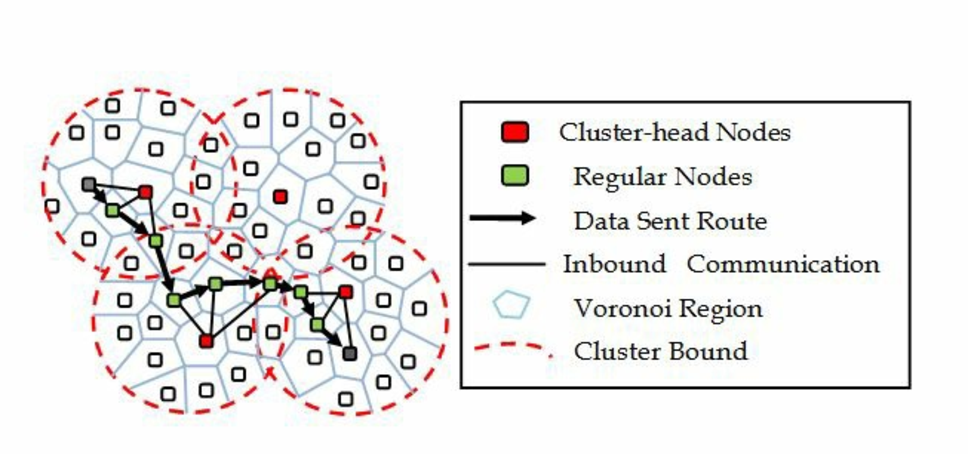
\includegraphics[width=0.84\linewidth]{fig2}
	\caption{Automatic reconfigurable deep neural network (ARDNN) architecture.}
	\label{fig:fig2}
\end{figure}


Our experimental results demonstrate that ARDNN can reduce computational cost to 1/30 with < 5\% accuracy degradation.
Therefore, ARDNN enables deep convolutional multi-layer neural networks to be run on resource-constrained CPSes,
thus opens the floodgate of novel industrial, automotive, security and consumer CPS applications.


\section{Future Work}

As this work is the first effort, to our best knowledge, to automatically re-configure DNN architecture,
we expect a lot of future research can be done, e.g., gauging the performance with different clustering granularity,
consideration of other deep-learning applications such as speech recognition, natural language processing.


\bibliographystyle{plain}
\begin{thebibliography}{10}

\bibitem{ref1}
C.~Alippi, ``Intelligence for Embedded Systems'',
{\em Springer Verlag},  283pp, ISBN 978-3-319-05278-6, 2014.

\bibitem{ref2}
White, Jules; Clarke, S.; Dougherty, B.; Thompson, C.; Schmidt, D.
``R\&D Challenges and Solutions for Mobile Cyber-Physical Applications and Supporting Internet Services''.
{\em Springer Journal of Internet Services and Applications}, 2010.

\bibitem{ref3}
Edward Lee, ``Cyber Physical Systems: Design Challenges'',
{\em University of California, Berkeley Technical Report} No. UCB/EECS-2008-8, 2008.

\bibitem{ref4}
Deng, L.; Yu, D., ``Deep Learning: Methods and Applications'',
{\em Foundations and Trends in Signal Processing}, 7: 3--4. doi:10.1561/2000000039, 2014.

\bibitem{ref5}
Bengio, Yoshua; LeCun, Yann; Hinton, Geoffrey,
``Deep Learning'', {\em Nature} 521: 436--444. doi:10.1038/nature14539, 2015.

\bibitem{ref6}
Khaitan et al.,
``Design Techniques and Applications of Cyber Physical Systems: A Survey'',
{\em IEEE Systems Journal}, 2014.

\end{thebibliography}

